%%%%%%%% ICML 2019 EXAMPLE LATEX SUBMISSION FILE %%%%%%%%%%%%%%%%%

\documentclass{article}

% Recommended, but optional, packages for figures and better typesetting:
\usepackage{microtype}
\usepackage{graphicx}
\usepackage{subfigure}
\usepackage{booktabs} % for professional tables

% hyperref makes hyperlinks in the resulting PDF.
% If your build breaks (sometimes temporarily if a hyperlink spans a page)
% please comment out the following usepackage line and replace
% \usepackage{icml2019} with \usepackage[nohyperref]{icml2019} above.
\usepackage{hyperref}

% Attempt to make hyperref and algorithmic work together better:
\newcommand{\theHalgorithm}{\arabic{algorithm}}

% Use the following line for the initial blind version submitted for review:
\usepackage[accepted]{icml2019}

% If accepted, instead use the following line for the camera-ready submission:
%\usepackage[accepted]{icml2019}

% The \icmltitle you define below is probably too long as a header.
% Therefore, a short form for the running title is supplied here:
% \icmltitlerunning{Submission and Formatting Instructions for ICML 2019}

\begin{document}

\twocolumn[
\icmltitle{Synthetic Data Generation for Security Applications\\
            Research Note}

% It is OKAY to include author information, even for blind
% submissions: the style file will automatically remove it for you
% unless you've provided the [accepted] option to the icml2019
% package.

% List of affiliations: The first argument should be a (short)
% identifier you will use later to specify author affiliations
% Academic affiliations should list Department, University, City, Region, Country
% Industry affiliations should list Company, City, Region, Country

% You can specify symbols, otherwise they are numbered in order.
% Ideally, you should not use this facility. Affiliations will be numbered
% in order of appearance and this is the preferred way.
\begin{icmlauthorlist}
\icmlauthor{Shengzhe Xu}{vt}
\icmlauthor{Manish Marwah}{hp}
\icmlauthor{Naren Ramakrishnan}{vt}
\end{icmlauthorlist}

\icmlaffiliation{vt}{Department of Computer Science, Virginia Tech, Arlington, USA}
\icmlaffiliation{hp}{Hewlett Packard Labs, USA}

\icmlcorrespondingauthor{}{}

\vskip 0.3in
]

% this must go after the closing bracket ] following \twocolumn[ ...

% This command actually creates the footnote in the first column
% listing the affiliations and the copyright notice.
% The command takes one argument, which is text to display at the start of the footnote.
% The \icmlEqualContribution command is standard text for equal contribution.
% Remove it (just {}) if you do not need this facility.

%\printAffiliationsAndNotice{}  % leave blank if no need to mention equal contribution
% \printAffiliationsAndNotice{\icmlEqualContribution} % otherwise use the standard text.

\begin{abstract}
In terms of novelty of approach, here are some ideas to pursue to differentiate from prior work:

- Use of side or auxiliary variables, such as time of day, day of week, location if available, etc.

- Shape of conv layer filter based on this application

- While there are no RBG channels, variables along a row are heterogeneous, and need to be models appropriately.

- Size of the problem - some IP addresses/users may have very large number of flows per hour; how do you handle that in an tractable manner, e.g, perhaps some sort of multi-scale, and/or hierarchical modeling

\end{abstract}

\section{Baseline Models}

We start our research from the UGR16 dataset: A New Dataset for the Evaluation of Cyclostationarity-Based Network IDSs.

\subsection{Data}
We first want to analyze and model data of April Week3 day 1. We filter out the flows that both Source Address and Target Address are internal ip (starting with 42.219.*.*), which are our current research target.

As a result, which is quite different with our previous outgoing traffic data (only filter SA with the internal ip pattern but not for DA), we got 732 users and 206300 flows from day 1 data. As shown in Figure 1 and the data\_stats.csv attachment file. In this data, 598 users have only 1 flow record. So we don't need to select users with medium \#flow as we planned for outgoing traffic data, but selected top 12 users. Figure 2 shows the \#flow of the 12 users in each hour of the day. Note that, top 2 users have much more \#flow than the other users, which may because they are server or port scanning something like we discussed last week. Thus, we tried to use the top 3-12 users to trained our model.

\begin{figure}[h]
\centering
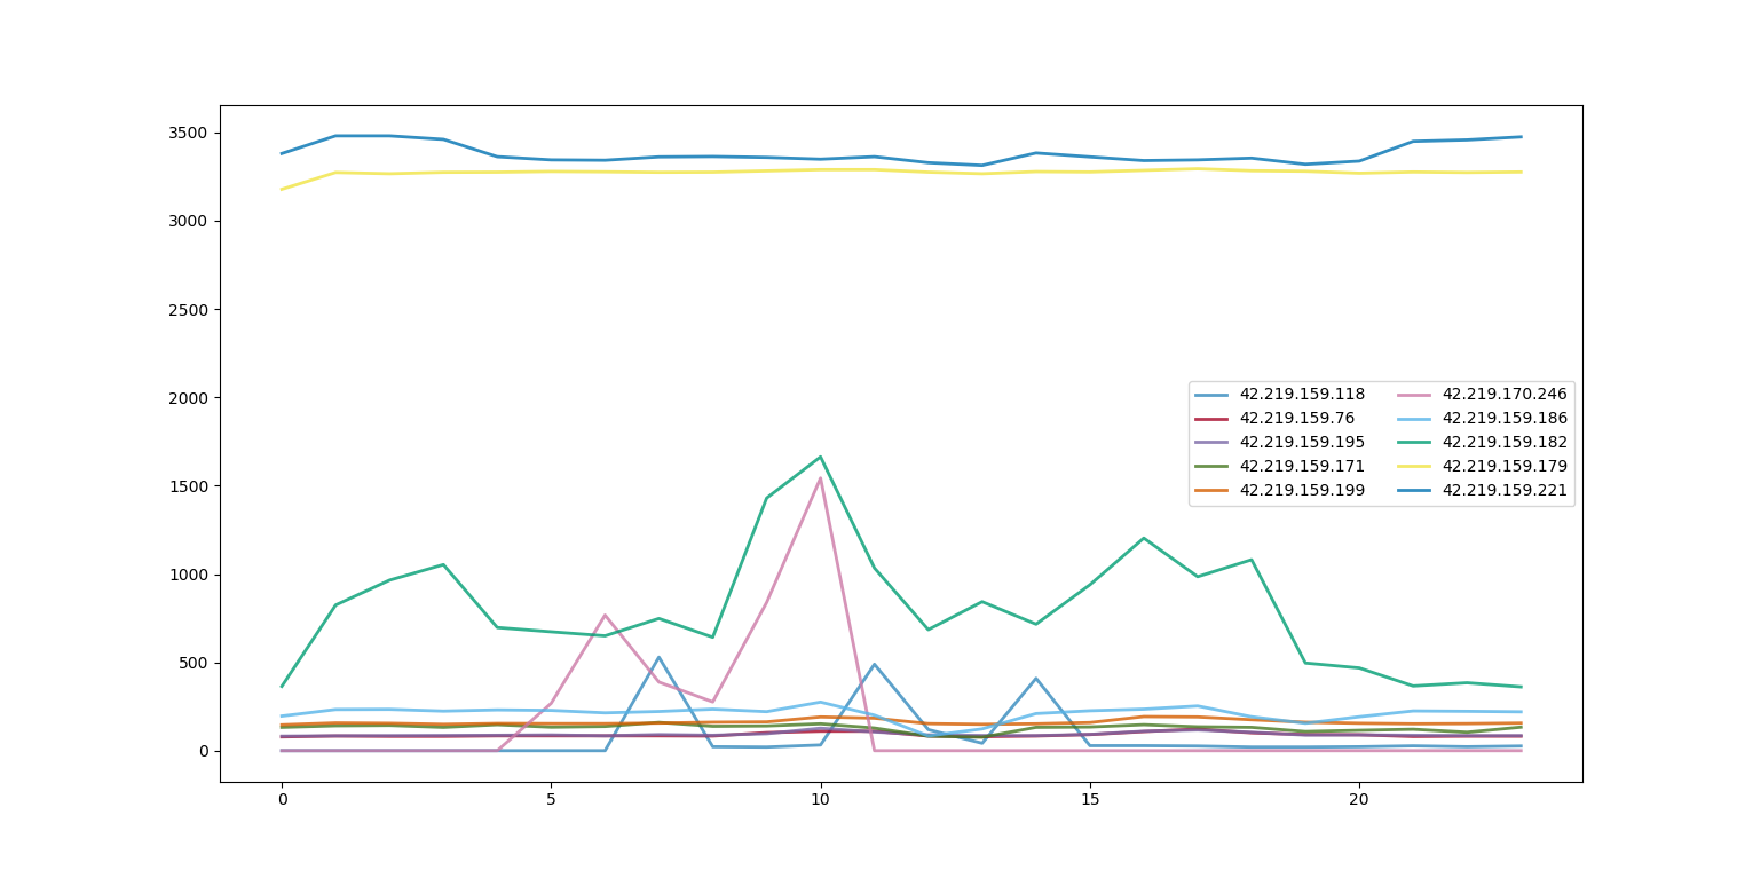
\includegraphics[width=0.5\textwidth]{figures/top1to10rawdatahourly.pdf}
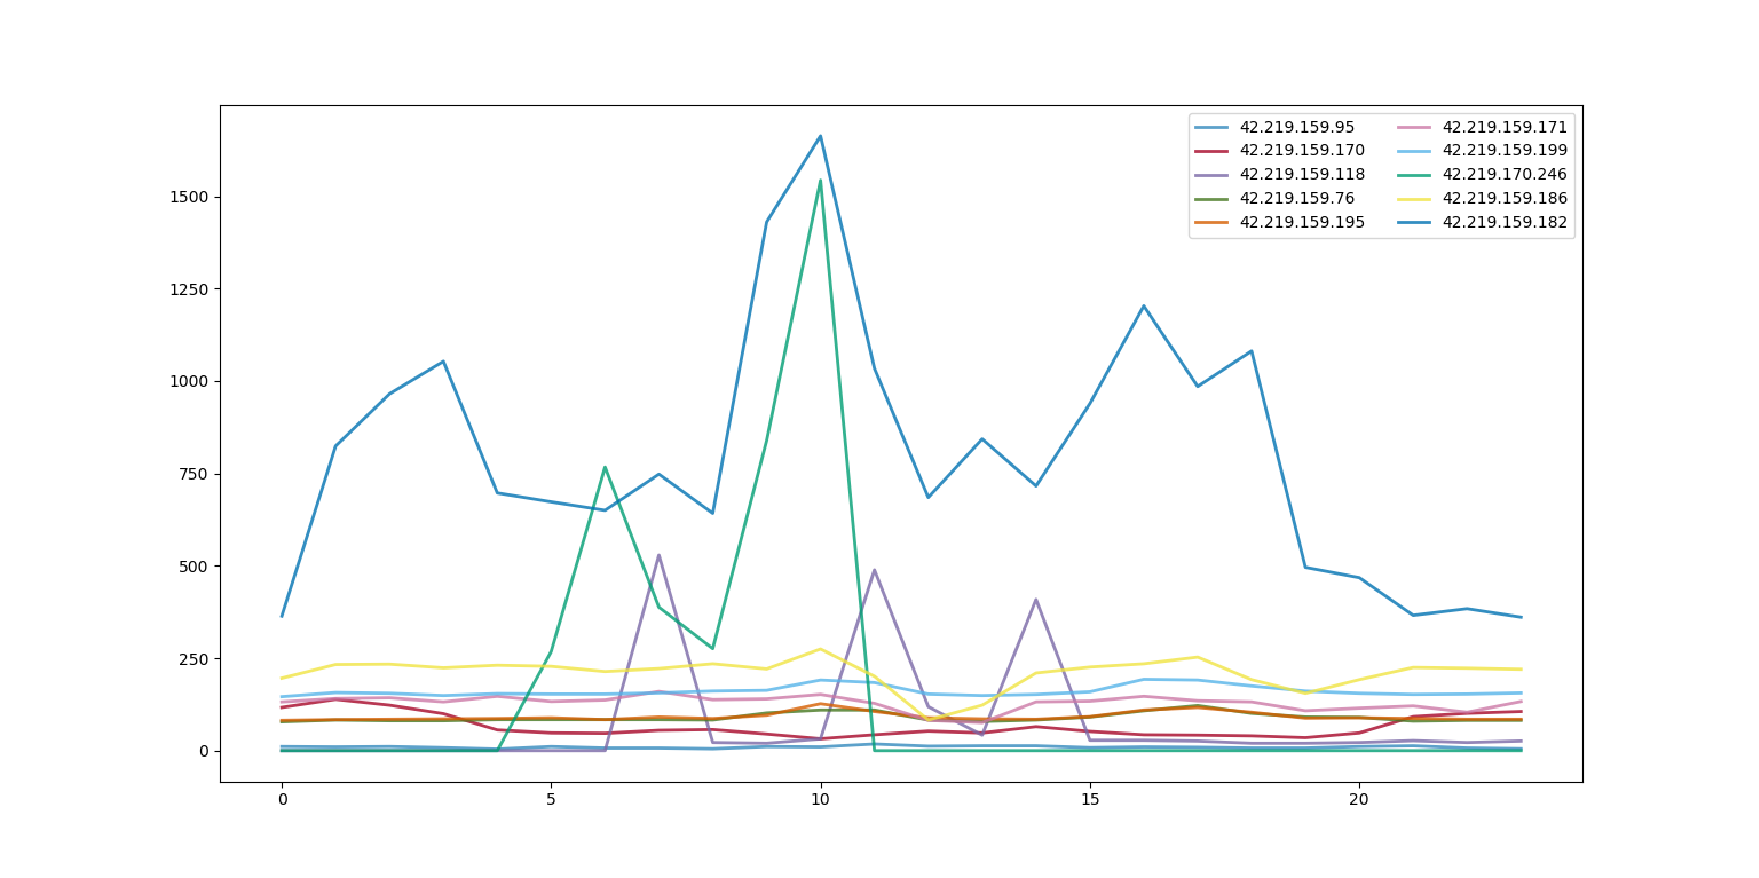
\includegraphics[width=0.5\textwidth]{figures/top3to12rawdatahourly.pdf}
\caption{top: hourly data for top 1st to 10th users; bottom: hourly data for top 3rd to 12th users}
\label{fig:hourly}
\end{figure}

(\textbf{Todo:} After filtering the flows in this way, the amount of the flows are not enough for the future deep learning. We can expand to data of multiple days for CNN model.)

(\textbf{Special Finding:} The \#byte of all flows of some users, like 42.219.170.246, are all 64)

\subsection{Baseline1: Independently model each column}
To describe.

\subsection{Baseline2: Naive Bayesian}

$argmax_{B}{P(B|T,(B-1))}, where P(B|T,(B-1)) = P(T|B) * P(B-1|B) * P(B)$

the bar problem is a trade off. Actually the p(x) can be expanded to p(x in bar) * p(bar in whole data).

To decide the bar, there are 2 potential solutions. First, use same-width bars. Second, use same-sample bars, which means we evenly put equal amount of sample in one bar. Both the 2 solutions ask us to decide the number of bars. May be we can enumerate and try different number of bar value on the training set, then select the best one.

\section{Result and Validation}
We generate a group of data and try to evaluate them.

\begin{tabular}{|c|c|c|c|}
 \hline
\#user & \#days & \#flows generated & model\\
 \hline
1 & 10 & 49648 rows & baseline1 \\
 \hline
1 & 10 & 49229 rows & baseline2 \\
 \hline
\end{tabular}

We want to use the cross-validation to evaluate the model we build. Like we should build the model from the raw data training set and then test the metrics between the raw data testing set and the model distribution. We make the use of the K-L divergence as well as the likelihood to be as our evaluation metrics.

\subsection{K-L divergence}
p(x) denote the distribution of the raw data and.

$D_{\mathrm{KL}} ( P \mathop{\|} Q ) = \sum_i P(i) \ln \left( \frac{P(i)}{Q(i)} \right).$

\textbf{all day data}
validation. 1. KL divergence of all day data.

\textbf{each hour data}

\subsection{Likelihood}
Since we model the data with the help of the Maximum Likelihood Estimate.

\section{Problems to be Dealt With}
The following link provides a theory that about the possible that p(i) and q(i) = 0.

https://math.stackexchange.com/questions/1228408/kullback-leibler-divergence-when-the-q-distribution-has-zero-values

https://stats.stackexchange.com/questions/275033/how-do-i-calculate-kl-divergence-between-two-multidimensional-distributions

% \bibliography{example_paper}
\bibliographystyle{icml2019}

\end{document}


% This document was modified from the file originally made available by
% Pat Langley and Andrea Danyluk for ICML-2K. This version was created
% by Iain Murray in 2018, and modified by Alexandre Bouchard in
% 2019. Previous contributors include Dan Roy, Lise Getoor and Tobias
% Scheffer, which was slightly modified from the 2010 version by
% Thorsten Joachims & Johannes Fuernkranz, slightly modified from the
% 2009 version by Kiri Wagstaff and Sam Roweis's 2008 version, which is
% slightly modified from Prasad Tadepalli's 2007 version which is a
% lightly changed version of the previous year's version by Andrew
% Moore, which was in turn edited from those of Kristian Kersting and
% Codrina Lauth. Alex Smola contributed to the algorithmic style files.
